\section{Results in three dimensions}
\label{sec:results3}

\subsection{Reproduction of the published record}

Table~\ref{tab:d3} lists the maximum found for $4 \leq n \leq 12$
\artref{cases} against the published value, which for $n = 10, 11$ is the
conjectural one \artref{catalog}, \artref{testcatalog}. Every row agrees
to at most $3 \times 10^{-15}$, and every optimum verifies as a convex-position
configuration whose combinatorial type matches the one recorded for it
\artref{testtables}.

\begin{table}[ht]
  \caption{Best values found on $\mathbb{S}^{2}$. ``Status'' refers to the
    published value, not to our computation.}
  \label{tab:d3}
  \begin{tabular}{rll l}
    \toprule
    $n$ & found & closed form & status \\
    \midrule
    4  & 0.513200239280 & $8\sqrt{3}/27$ & proven \\
    5  & 0.866025403784 & $\sqrt{3}/2$ & proven \\
    6  & 1.333333333333 & $4/3$ & proven \\
    7  & 1.585094193825 & $(5/3)\sin(2\pi/5)$ & proven \\
    8  & 1.815716104224 & $\sqrt{(475 + 29\sqrt{145})/250}$ & proven \\
    9  & 2.043750115900 & $3\sqrt{2\sqrt{3}-3}$ & proven \\
    10 & 2.218711131545 & $16\bigl(3 + \sqrt{2} +
         \sqrt{38 + 6\sqrt{2}}\bigr)/81$ & conjectural \\
    11 & 2.354634495069 & --- & conjectural \\
    12 & 2.536150710120 & $(2/3)\sqrt{10 + 2\sqrt{5}}$ & proven \\
    \bottomrule
  \end{tabular}
\end{table}

At $n = 9$ simpliciality (Lemma~\ref{lem:propertyz}) is what keeps the
enumeration small: Hoehner and Ledford reduce the $2606$ combinatorial types of nine-vertex polyhedra to the
$50$ simplicial ones \cite{hoehner-ledford-2026}, and \texttt{plantri}
generates exactly those $50$. Maximising within each gives the triaugmented
triangular prism, $3\sqrt{2\sqrt{3}-3}$, shown in Figure~\ref{fig:d3n09}.
Symmetry detection returns a group of order $12$, six proper and six improper
elements with orbits of sizes $3$ and $6$, that is $D_{3h}$; we read it off the
maximiser reconstructed from the closed-form coordinates of
\cite{hoehner-ledford-2026}, because the swept optimum is congruent to that
configuration only to about $5 \times 10^{-8}$ and at the $10^{-7}$ Gram tolerance of
Section~\ref{sec:method} resolves only an order-$2$ subgroup \artref{testtables}.

\begin{figure}[ht]
  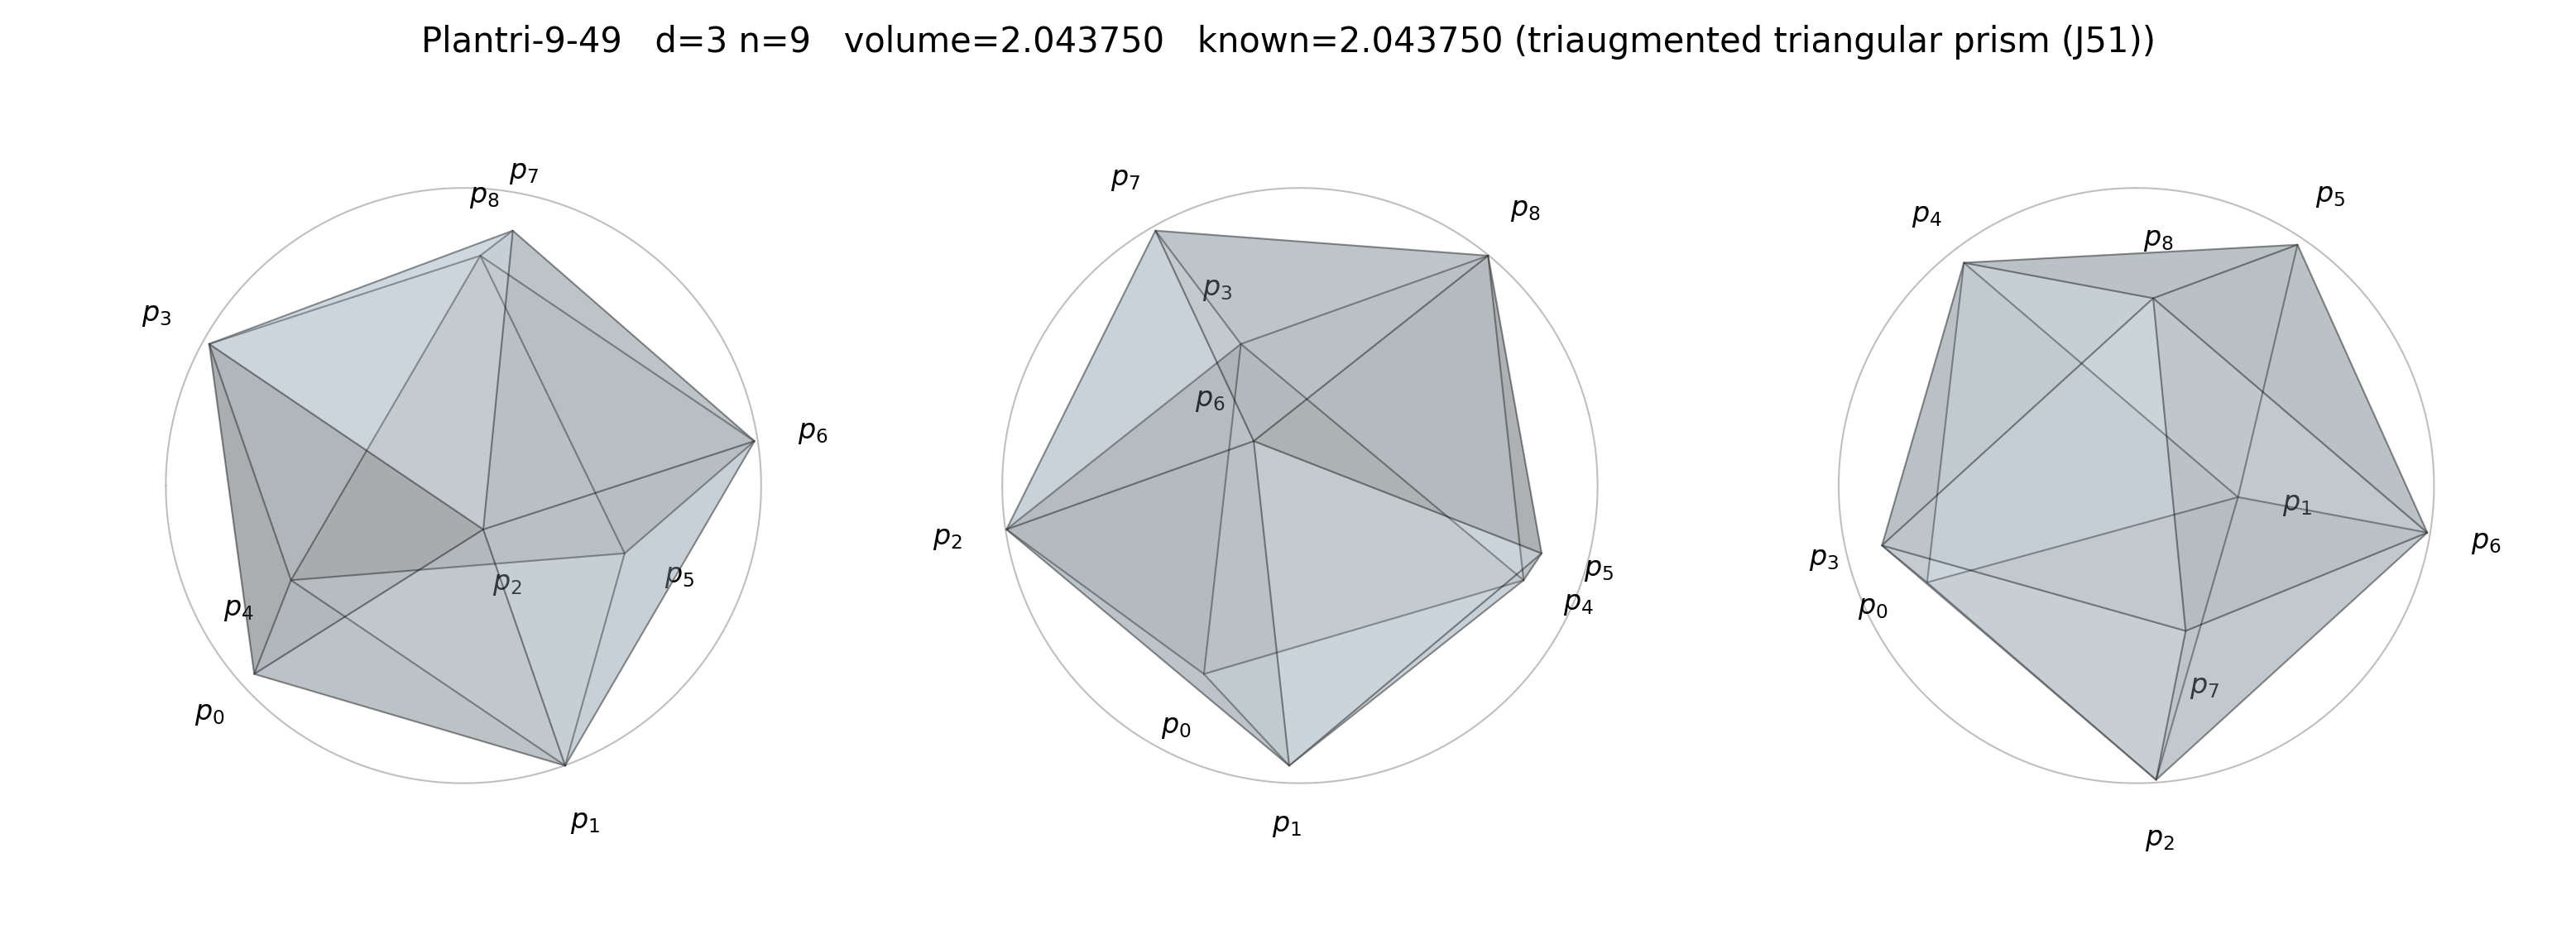
\includegraphics[width=\textwidth]{d3-n09.png}
  \caption{The $n = 9$ maximiser, three views. Vertices $p_{0},\dots,p_{8}$ on
    $\mathbb{S}^{2}$; the type is \texttt{plantri-9-49}, the triaugmented
    triangular prism.}
  \label{fig:d3n09}
\end{figure}

\subsection{Triage}

The relaxation triage of Section~\ref{sec:triage} behaves very differently
across this range \artref{cases}. Writing rivals for the non-winning types of a
case:

\begin{center}
\begin{tabular}{lrrrrrrrrr}
  \toprule
  $n$ & 4 & 5 & 6 & 7 & 8 & 9 & 10 & 11 & 12 \\
  \midrule
  rivals & 0 & 0 & 1 & 4 & 13 & 49 & 232 & 1248 & 7594 \\
  hard   & 0 & 0 & 0 & 0 & 0  & 3  & 40  & 584  & 5375 \\
  level  & E1 & E1 & E3 & E3 & E3 & E1 & E1 & E1 & E1 \\
  \bottomrule
\end{tabular}
\end{center}

At $n = 6, 7, 8$ every rival is excludable, so these cases reach E3. At $n = 4$
and $n = 5$ the enumeration holds a single type, so there is no rival to
exclude and the case stays at E1 however complete it is. From $n = 9$ onwards
the hard set is non-empty and E3 is unavailable; the heptagonal bipyramid of
Section~\ref{sec:trap} is one of the three hard types there. By $n = 11$ the
relaxation fails to separate $584$ of $1248$ rivals.

The $n = 12$ sweep covers all $7595$ types, including those with a degree-3
vertex, and returns the icosahedron \artref{cases}. Its $31$ feasible types
include $9$ with a degree-3 vertex, the largest of them at $2.370904$, so
restricting to minimum degree $4$ would have discarded inscribed polytopes and
not folds alone \artref{testtables}.
